\documentclass[a4paper]{article}
    \usepackage{minted}
    \usepackage{xcolor}
    \usepackage[colorlinks,linkcolor=black]{hyperref}
    \usepackage[margin=1in]{geometry}
    \usepackage{caption}
    \usepackage{graphicx, subfig}
    \usepackage{float}
    \definecolor{bg}{rgb}{0.9,0.9,0.9}
    \usemintedstyle{manni}
    \setminted{
    linenos,
    autogobble,
    breaklines,
    breakautoindent,
    bgcolor=bg,
    numberblanklines=false,
    }

\begin{document}
    \tableofcontents
    \newpage
    \section{Problem Description}
        \subsection{Exercise 1}
Implement home.php with a text input box and a search button, which sends the input content to result.php using a GET request on the click.
        \subsection{Exercise 2}
Implement result.php, which displays the first 10 matching scholars in descending order of the number of papers. The main affiliation of each scholar and the hyperlink to the scholar's page should also be displayed.
        \subsection{Exercise 3}
Implement author.php, which displays the 10 most cited papers of the author. For every paper, its venue and authors in sequence should also be displayed. Like Exercise 1, the hyperlink to the author's page is needed.
        \subsection{Exercise 4}
Add the function of autocomplete to the text input box of home.php and implement hint.php, which receives the real-time input from home.php and returns hints for autocomplete.
        \subsection{Exercise 5 (Optional)}
Migrate all the PHP code above to the framework CodeIgniter and do proper MVC seperation.
    \section{Problem Analysis}
        \subsection{Skills Involved}
These exercises mainly involves the knowledge of PHP and SQL for the backend. Besides, some basic understanding of HTML and CSS would help do the part of display.

As for the optional exercise, the skills of developing with the framework CodeIgniter are also required.
        \subsection{Solution Design}
Considering the huge difference of two solutions (Raw PHP and CodeIgniter), solution design will be stated seperatedly in the following two sections.

    \section{Solution One : Raw PHP}
        \subsection{home.php}
            \subsubsection{Form}
Just with some basic knowledge of HTML, the form can be easily implemented. The code for the form is as follows:
                \begin{minted}{html}
        <form action="result.php" method="get">
            <input type="text" id="authorname" name="authorname">
            <input type="submit" id="homeSubmit" value="Search">
        </form>
                \end{minted}
            \subsubsection{Autocomplete}
According to the instructions, the Autocomplete widget of jQuery can be applied for this task. But as the given tutorial is nearly 7 years ago, it's been outdated and can't work properly.

Therefore, I switch to the latest version of Jquery UI and use a slightly different method. Instead of downloading the Jquery UI files, I just link to its CDN.

The code for autocomplete is as follows:
                \begin{minted}{html}
    <link rel="stylesheet" href = "https://code.jquery.com/ui/1.12.1/themes/base/jquery-ui.css" >
    <script src="https://code.jquery.com/jquery-1.12.4.js"> </script>
    <script src="https://code.jquery.com/ui/1.12.1/jquery-ui.js"> </script>
    <script type="text/javascript">
        $(function(){
            $( "#authorname" ).autocomplete({
                source: "hint.php",
                minLength: 1,
            });
        });
    </script>
                \end{minted}
        \subsection{connect.php}
As in different PHP files, connection to the database is frequently needed, it's better to write it in a single PHP file connect.php to simplify other files.

There're sereval ways for PHP applications to connect to MySQL database, and I choose to use MySQLi, which is object-oriented. The code is like these:
            \begin{minted}{php}
<?php
    $servername="...";  //omitted
    $username="...";
    $password="...";
    $database="...";
    $conn=new mysqli($servername,$username,$password,$database);
    if($conn->connect_error){
        die("Failed to connect to the database:".$conn->connect_error);
    }
 ?>
            \end{minted}
        \subsection{hint.php}
            \subsubsection{SQL Query}
As required, hint.php receives the parameter term and searches in the database for matching authors. So it needs to connect to the database and execute SQL queries to get the search result.

The SQL query is designed like this:
                \begin{minted}{sql}
SELECT authors.*,paper_author_affiliation.num
FROM authors,
    (SELECT authorid,count(1) AS num FROM paper_author_affiliation GROUP BY authorid)paper_author_affiliation
WHERE authors.authorid=paper_author_affiliation.authorid AND authors.authorname LIKE '%$authorname%'
ORDER BY num DESC
LIMIT 10;
                \end{minted}
And the complete code will be shown at the end of this section.
            \subsubsection{Json}
The Autocomplete widget of jQuery UI works in a way that requires hint.php to return Json encoded information, so the final step of hint.php is to encode the result into Json code.

With the help of the built-in function json\_encode(), things are relatively easy.
                \begin{minted}{php}
echo json_encode($resultArray);
                \end{minted}
            \subsubsection{The Complete Code}
Things to note are that we include connect.php to do the job of connecting to the database with MySQLi and that fileter\_input() function makes sure that there's no illegal character in authorname to avoid potential security risks.
                \begin{minted}{php}
<?php
    if(filter_has_var(INPUT_GET, "term")){
        include_once("connect.php");
        $authorname=filter_input(INPUT_GET, "term",FILTER_SANITIZE_MAGIC_QUOTES);
        $authorname=strtolower($authorname);
        $query="..."; //omiited as it has been shown before
        $queryResult=$conn->query($query);
        while($row = $queryResult->fetch_assoc()) {
            $resultArray[] = array('id' => $row["AuthorID"],'label'=>$row["AuthorName"] );
        }
        echo json_encode($resultArray);
    }
?>
                \end{minted}
        \subsection{result.php}
            \subsubsection{SQL Query}
In result.php, given the author's name, we do the fuzzy search to get the 10 most cited authors and their main affiliation.

Maybe things can be done in a single SQL query, but for simplicity and clearness, I choose to divide the query into two steps:

First, get the 10 most cited authors. The SQL query is like this:
                \begin{minted}{sql}
SELECT authors.*,paper_author_affiliation.num
FROM authors,
    (SELECT authorid,count(1) AS num FROM paper_author_affiliation GROUP BY authorid)paper_author_affiliation
WHERE authors.authorid=paper_author_affiliation.authorid AND authors.authorname LIKE '%$authorname%'
ORDER BY num DESC
LIMIT 10;
                \end{minted}
Second, for each author, get his/her main affiliation. The SQL query is like this:
                \begin{minted}{sql}
SELECT affiliations.*
FROM affiliations,
    (SELECT affiliationid,count(1)
        FROM paper_author_affiliation
        WHERE authorid='$authorID'
        GROUP BY affiliationid
        ORDER BY count(1) DESC)paper_author_affiliation
WHERE affiliations.affiliationid = paper_author_affiliation.affiliationid
LIMIT 1;
                \end{minted}
            \subsubsection{Display}
Considering the structure of data, using table is a simple way to present the result. The code for the table is like these:
            \begin{minted}{html}
<table id='searchResult' align='center'>
    <tr>
        <th>Author Name</th>
        <th id="widenColumn">Total Citations</th>
        <th>Affiliation Name</th>
    </tr>
        <tr>
        <td ><a href='/author.php?authorid=77487C6A'>Johannes Asfalg</a></td>
        <td id='widenColumn'>1</td>
        <td >
            <ul><li>
            <a href='/affiliation.php?affiliationid=007D2F41' >
                Ludwig Maximilian University Of Munich
            </a>
            </li></ul>
        </td>
    </tr>
</table>
            \end{minted}
And if the authorname is not given or there's no result found, it shows an error page, of which the code is like these:
            \begin{minted}{php}
<?php
if(isset($_GET['authorname'])){
    //omitted
}else{
    echo "<div id='noResult'>Invalid Author Name!</div>";
}
?>
            \end{minted}
Note that in the above two code snippets, I use some CSS ID selectors defined in the file css/main.css, which will be further explained in the last subsection of this section.
        \subsection{author.php}
            \subsubsection{SQL Query}
For author.php, the SQL query is more complicated, so still, dividing the query into some steps is a good idea.

First, we check whether the authorid exists:
                \begin{minted}{php}
<?php
$queryForExistence="SELECT count(1) as num FROM paper_author_affiliation WHERE authorID = '$authorID'";
$queryResultForExistence=$conn->query($queryForExistence);
$row=$queryResultForExistence->fetch_assoc();
if($row["num"]==0)
    echo "<div id='noResult'>No Paper Founded!</div>";
?>
                \end{minted}
Second, Having confirmed the existence, we query for author's name:
                \begin{minted}{php}
<?php
$queryForName="SELECT AuthorName From authors where AuthorID='$authorID'";
$queryResultForName=$conn->query($queryForName);
$authorName=($queryResultForName->fetch_assoc())["AuthorName"];
?>
                \end{minted}
Third, query for the 10 most cited papers of the author:
                    \begin{minted}{php}
<?php
$queryForPaper="
SELECT papers.*,conferences.ConferenceName,paper_reference.citation
FROM papers,conferences,paper_author_affiliation,
    (SELECT referenceid,count(1) AS citation FROM paper_reference GROU)paper_reference
WHERE papers.paperid = paper_reference.referenceid
    AND conferences.conferenceid = papers.conferenceid
    AND papers.paperid = paper_author_affiliation.paperid
    AND paper_author_affiliation.authorid = '$authorID'
ORDER BY citation DESC
LIMIT 10;";
$paperCnt=0;
$queryResultForPaper=$conn->query($queryForPaper);
while($row=$queryResultForPaper->fetch_assoc()){
    $paperCnt++;
    handleOnePaper($row,$conn);
}
?>                   \end{minted}
Fourth, for every paper, query for its authors, which is a part of the function handleOnePaper():
                    \begin{minted}{sql}

SELECT authors.AuthorName,paper_author_affiliation.*
FROM authors, ( SELECT * FROM paper_author_affiliation WHERE paperid='$paperID'paper_author_affiliation
WHERE paper_author_affiliation.authorid=authors.authorid
ORDER BY paper_author_affiliation.authorsequence ASC;
                    \end{minted}
Lastly, note that in the above procedures every paper we get is cited at least once, that's to say, we leave behind the papers with no citation. This could cause problems if the author has less than 10 cited papers.

So, an additional query is needed if in the third step we get less than 10 papers:
                    \begin{minted}{php}
<?php
if($paperCnt<10){
$extraNum=10-$paperCnt;
$queryForExtraPaper="
SELECT papers.*,conferences.ConferenceName
FROM papers,conferences,paper_author_affiliation
WHERE papers.paperid=paper_author_affiliation.paperid
    AND paper_author_affiliation.authorid='$authorID'
    AND (Select count(1) FROM paper_reference WHERE paper_reference.referenceid = papers.paperid) = 0
    AND papers.conferenceid=conferences.conferenceid
LIMIT $extraNum;";
$queryResultForExtra=$conn->query($queryForExtraPaper);
while($row=$queryResultForExtra->fetch_assoc()){
    $paperCnt++;
    handleOnePaper($row,$conn,$noCitation=true);
}
?>
                    \end{minted}
            \subsubsection{Display}
The same as the display of the search result, I choose to use a table to present the papers and use a ordered list for authors.
                \begin{minted}{html}
<table id='papers' align='center'>
    <tr>
        <th id="narrowedColumn">Paper Title</th>
        <th>Publish Year</th>
        <th>Conference</th>
        <th>Citations</th>
        <th style="text-align:center">Author(s)</th>
    </tr>

    <tr>
        <td id = "narrowedColumn"> Querying Inconsistent Description Logic Knowledge Bases Under Preferred Repair Semantics </td>
        <td>2014</td>
        <td>AAAI</td>
        <td>1</td>
        <td>
            <ol>
                <li>
                    <a href="/author/7F4D1062">Meghyn Bienvenu</a>
                </li>
                <li>
                    <a href="/author/7DA12C4C">Camille Bourgaux</a>
                </li>
                <li>
                    <a href="/author/01E80BB2">Francois Goasdoue</a>
                </li>
            </ol>
        </td>
    <tr>
</table>
                \end{minted}
For tha sake of beauty and completeness, I also add the image and description of tha author.
                    \begin{minted}{html}
<img id="photo" src="/static/img/author.jpg">
<div id="profile">
    <p>
This is the description. This is the description.This is the description.
This is the description. This is the description. This is the description.
This is the description. This is the description.
    </p>
    <p>
This is the description. This is the description.This is the description.
This is the description. This is the description. This is the description.
This is the description. This is the description.
    </p>
</div>
                    \end{minted}
        \subsection{main.css}
As we need to customize the appearence of pages, using a CSS file saves unnecessary code and is easy to modify and migrate to other soulutions. For example, the style for empty result and hyperlinks are like these:
                    \begin{minted}{css}
#noResult{
    font-size:30px;
    color: gray;
    margin-top: 50px;
    position: absolute;
    left: 50%;
    transform: translate(-50%,0);
}
a:link {
    text-decoration: none;
}
a:visited {
    text-decoration: none;
}
a:hover {
    text-decoration: none;
}
a:active {
    text-decoration: none;
}
                    \end{minted}

    \section{Solution Two : CodeIgniter}
        \subsection{Overall Design And Config}
As I have solved all the problems with Solution One already, many things can be reused. For instance, the CSS file, SQL queries, and HTML code just need to be modified rather than rewrote.

With these, I just need to consider how to seperate this PHP appilication into Model, View and Controller properly, which will be covered in the following subsections.

To get the framework CodeIgniter to work, the first thing is to configure it properly. Files in application/config such as config.php and database.php need to be modified.

        \subsection{Model}
            \subsubsection{Search Result Model}
Considering the similarity of SQL queries between hint.php and result.php of Solution One, they can be integrated into one model extending from CI\_Model, Search\_result\_model in application/models /Search\_result\_model .php.

On construction, it loads the database.
                \begin{minted}{php}
<?php
    public function __construct()
    {
        $this->load->database();
    }
?>
                \end{minted}
Then it has two public functions for hint and search result respectively: get\_hint() and get\_search\_result(), in which the SQL queries are simialr to those of Solution One and omitted in the following code.
                \begin{minted}{php}
<?php
    public function get_hint($authorname=NULL)
    {
        $query=$this->db->query("..."); //omitted here
        return $query->result_array();

    }
    public function get_search_result($authorname="",$begin=0,$end=10)
    {
        $queryForAuthor=$this->db->query("...");    //omitted here
        if(!$queryForAuthor->result_array())
            return NULL;
        else{
            $result=array();
            foreach($queryForAuthor->result_array() as $row){
                $singleAuthor["authorID"]=$row["AuthorID"];
                $singleAuthor["authorName"]=$row["AuthorName"];
                $singleAuthor["paperNum"]=$row["num"];
                $queryForAffiliation=$this->db->query("...");   //omitted here
                $rowAff=$queryForAffiliation->row_array();
                $singleAuthor["affiliationID"]=$rowAff["AffiliationID"];
                $singleAuthor["affiliationName"]=$rowAff["AffiliationName"];
                array_push($result, $singleAuthor);
            }
            return $result;
        }
    }
?>
                \end{minted}
            \subsubsection{Author Info Model}
This model is specificly designed for getting an author's information like name, image, description and papers.

Its main member function is get\_author\_info(), which takes an author ID and returns all the information about the author. Again, as the SQL queries are similar to previous ones in Solution One, they are omitted in the code.
                \begin{minted}{php}
<?php
    public function get_author_info($authorID=NULL,$maxPaperNum=10)
    {
        $queryForExistence=$this->db->query("..."); //omitted here
        if($queryForExistence->row_array()["num"]==0)
            return NULL;
        $result=array();
        $queryForName=$this->db->query("..");   //omitted here
        $result["authorName"]=($queryForName->row_array())["AuthorName"];
        $result["authorDescription"]="...";
        $result["authorImg"]="...";
        $queryForPaper=$this->db->query("...");    //omitted here
        $paperCnt=0;
        $papers=array();
        foreach ($queryForPaper->result_array() as $row) {
            $paperCnt+=1;
            array_push($papers, $this->handle_one_paper($row));
        }
        if($paperCnt<10){
            $extraNum=10-$paperCnt;
            $queryForExtraPaper=$this->db->query("...");    //omitted here
            foreach ($queryForExtraPaper->result_array() as $row) {
                $paperCnt+=1;
                $row["citation"]=0;
                array_push($papers, $this->handle_one_paper($row));
            }
        }
        $result["papers"]=$papers;
        return $result;
    }
?>

                \end{minted}
Two auxiliary functions are also defined for convenience: handle\_one\_paper()(as you see in the above code) and get\_paper\_author().

Note that handle\_one\_paper() is private as it has no value for outside callers and get\_paper\_author() is public as it has the potential to be reused.
                \begin{minted}{php}
<?php
    private function handle_one_paper($row)
    {
        $temp["paperID"]=$row["PaperID"];
        $temp["paperTitle"]=$row["Title"];
        $temp["paperPublishYear"]=$row["PaperPublishYear"];
        $temp["conferenceID"]=$row["ConferenceID"];
        $temp["conferenceName"]=$row["ConferenceName"];
        $temp["citation"]=$row["citation"] ?? 0;
        $temp["authors"]=$this->get_paper_author($row["PaperID"]);
        return $temp;
    }

    public function get_paper_author($paperID=NULL)
    {
        $queryForAuthors=$this->db->query(".."); //omitted here
        $authors=array();
        foreach ( $queryForAuthors->result_array() as $subAuthor) {
            $temp["subAuthorName"]=$subAuthor["AuthorName"];
            $temp["subAuthorID"]=$subAuthor["AuthorID"];
            $temp["subAuthorSequence"]=$subAuthor["AuthorSequence"];
            array_push($authors, $temp);
        }
        return $authors;
    }
?>
                \end{minted}
        \subsection{View}
            \subsubsection{Header, Footer and Error Template}
As all HTML pages contain some common code, putting it in templates is a feasible idea. So the header, footer and error page can be put in the folder application/views/templates. For example, header.php is as follows:
                \begin{minted}{html}
<!DOCTYPE html>
<html lang="en">
<head>
    <meta charset="UTF-8">
    <title><?php echo $title; ?></title>
    <link rel="stylesheet" href="/static/css/main.css">
</head>
<body>
    <h1><?php echo $title; ?></h1>
                \end{minted}
            \subsubsection{Home Page}
Considering the uniqueness of home page, it's hard for it to use the previous header and footer. So I just create a template for it, home.php.
                \begin{minted}{html}
<!DOCTYPE html>
<html lang="en">
<head>
    <meta charset="UTF-8">
    <title>Home</title>
    <link rel="stylesheet" href="/static/css/main.css">
    <link rel="stylesheet" href="https://code.jquery.com/ui/1.12.1/themes/base/jquery-ui.css">
    <script src="https://code.jquery.com/jquery-1.12.4.js"></script>
    <script src="https://code.jquery.com/ui/1.12.1/jquery-ui.js"></script>
    <script type="text/javascript">
        $(function(){
            $( "#authorname" ).autocomplete({
                source: "hint.php",
                minLength: 1,
            });
        });
    </script>
</head>
<body>
    <div id="superCenter">
    <h1>Home</h1>

    <div id="homepage" align="center">
        <?php echo form_open('/'); ?>
            <input type="text" id="authorname" name="authorname">
            <input type="submit" id="homeSubmit" value="Search">
        </form>
    </div>
    </div>

</body>
</html>
                \end{minted}
Note that Line 23 of the code snippet is a little unusual, which will be explained in the subsection Controller.
            \subsubsection{Search Result Page}
Search result page takes data from the controller and presents them in HTML. As CodeIgniter allows the template file to be a mixture of HTML and PHP, it looks like these:
                \begin{minted}{php}
<?php
    function echoAuthor($authorID,$authorName,$paperNum,$affiliationID,$affiliationName)
    {
        $affiliationName=$affiliationName ?ucwords($affiliationName): "None";
        $affiliationID=$affiliationID??"00000000";
        $authorName=ucwords($authorName);
        echo "
    <tr>
        <td ><a href='/author/$authorID'>$authorName</a></td>
        <td id='widenColumn'>$paperNum</td>
        <td ><ul><li><a href='/affiliation/$affiliationID'>$affiliationName</a></li></ul></td>
    </tr>\n";
    }
?>

<table id='searchResult' align='center'>
    <tr>
        <th>Author Name</th>
        <th id="widenColumn">Total Citations</th>
        <th>Affiliation Name</th>
    </tr>
    <?php
    foreach ($searchResult as $singleAuthor) {
        echoAuthor($singleAuthor["authorID"], $singleAuthor["authorName"], $singleAuthor["paperNum"], $singleAuthor["affiliationID"], $singleAuthor["affiliationName"]);
    }
    ?>
</table>
                \end{minted}
            \subsubsection{Author Page}
Similar to the search result page, the template file looks like these:
                \begin{minted}{php}
<img id="photo" src="<?php echo $author_info['authorImg']; ?>">
<div id="profile">
    <?php echo $author_info["authorDescription"]; ?>
</div>
<?php
    if(!$author_info["papers"]){
        echo "<div id='noResult'>No Paper Founded!</div>";
        exit();
    }
?>
<table id='papers' align='center'>
    <tr>
        <th id="narrowedColumn">Paper Title</th>
        <th>Publish Year</th>
        <th>Conference</th>
        <th>Citations</th>
        <th style="text-align:center">Author(s)</th>
    </tr>
<?php
    foreach ($author_info["papers"] as $paper) {
        echo '
    <tr>
        <td id="narrowedColumn">'.ucwords($paper["paperTitle"]).'</td>
        <td>'.$paper["paperPublishYear"].'</td>
        <td>'.$paper["conferenceName"].'</td>
        <td>'.$paper["citation"].'</td>
        <td>
            <ol>';
        foreach($paper["authors"] as $subAuthor){
            echo '
                <li>
                    <a href= "/author/'.$subAuthor["subAuthorID"].'">'.ucwords( $subAuthor["subAuthorName"] ).'</a>
                </li>';
        }
        echo '
            </ol>
        </td>';
    }
?>
</table>
                \end{minted}
        \subsection{Controller}
As this application is quite light, I only define a controller Page extending from CI\_Controller with several methods as follows.
            \subsubsection{index()}
This method is for the home page, in which there's a form for input. To implement the from, it needs to load the form helper and form\_validation. Also, as mentioned in the subsection View, the view of home page needs to create the form in this way:
                \begin{minted}{php}
<?php echo form_open('/'); ?>
                \end{minted}
If the data in the form pass the validation, then it redirects to the result page. Otherwise, just stay in the home page. So the code snippet is like these:
                \begin{minted}{php}
<?php
    public function index()
    {
        $this->load->helper('form');
        $this->load->library('form_validation');
        $this->form_validation->set_rules('authorname', 'Author Name', 'required');
        if ($this->form_validation->run() === FALSE){
            $this->load->view('templates/home.php');
        }
        else{
            $authorName=$this->input->post("authorname");
            redirect("/result/$authorName");
        }
    }
?>
                \end{minted}
            \subsubsection{result()}
This method is for the search result page. It first checks whether the parameter authorname is set and if not, loads the error page. Else, it gets the search result from Search\_result\_model() and transfers the data to the view, result.php.
                \begin{minted}{php}
<?php
    public function result($authorname=NULL)
    {

        if(!$authorname){
            $data["title"]="Error";
            $data["errorMsg"]="Invalid Author Name!";
            $this->load->view("templates/header.php",$data);
            $this->load->view("templates/error.php",$data);
            $this->load->view("templates/footer.php");
        }else{
            $authorname=str_replace("%20", " ", $authorname);
            $data["title"]="Result of ".ucwords($authorname);
            $data["searchResult"]=$this ->Search_result_model ->get_search_result($authorname);
            $this->load->view("templates/header.php",$data);
            if(!$data["searchResult"]){
                $data["errorMsg"]="No Author Found!";
                $this->load->view("templates/error.php",$data);
            }else{
                $this->load->view("templates/result.php",$data);
            }
            $this->load->view("templates/footer.php");
        }
    }
?>
                \end{minted}
            \subsubsection{author()}
This method works very similar to result(), both getting data from the model and transferring data to the corresponding view.
                \begin{minted}{php}
<?php
    public function author($authorID=NULL)
    {
        if(!$authorID){
            $data["title"]="Error";
            $data["errorMsg"]="Invalid Author ID!";
            $this->load->view("templates/header.php",$data);
            $this->load->view("templates/error.php",$data);
            $this->load->view("templates/footer.php");
        }else{
            $data["author_info"]=$this ->Author_info_model ->get_author_info($authorID);
            if($data["author_info"]==NULL){
                $data["title"]="Error";
                $data["errorMsg"]="Invalid Author ID!";
                $this->load->view("templates/header.php",$data);
                $this->load->view("templates/error.php",$data);
            }else{
                $data["title"]=ucwords($data["author_info"]["authorName"])."'s Page";
                $this->load->view("templates/header.php",$data);
                $this->load->view("templates/author.php",$data);
            }
            $this->load->view("templates/footer.php");

        }
    }
?>
                \end{minted}
        \subsection{Route}
The URL pattern looks like http://example.com/index.php/page/author/00000000, which is a little too complicated. To simplify the URL, we need to modify config/routes.php.

First, to eliminate the unnecessary "/page", we just set the default\_controller as Page and add rules for routes like these:
            \begin{minted}{php}
<?php
    $route['default_controller'] = 'page';
    $route['result/(:any)']='page/result/$1';
    $route['author/(:any)']='page/author/$1';
    $route['(:any)'] = 'page/$1';
?>
            \end{minted}
Then the URL may look like http://example.com/index.php/author/00000000, still having the unnecessary "/index.php".

To get rid of it, we need to let Apache allow override and put the file .htaccess in the folder of CodeIgniter, of which the content is:
            \begin{minted}{html}
RewriteEngine On
RewriteCond %{REQUEST_FILENAME} !-f
RewriteCond %{REQUEST_FILENAME} !-d
RewriteRule ^(.*)$ index.php/$1 [L]
            \end{minted}
And in config.php, set
            \begin{minted}{php}
<?php
$config['index_page'] = '';
?>
            \end{minted}
Having done all these, the URL finally looks like http://example.com/author/00000000.

Pretty!
        \subsection{Some Critical Issues}
            \subsubsection{Autocomplete}
What we have done in Solution One should work fine in CodeIgniter, but there's one critical problem:
/hint.php?term=something can't been handled directly by CodeIgniter, as the standard URL pattern is /class/method/arguments.

To solve this, there are two possible ways:

First, configure CodeIgniter to enable query strings, which is natural but a little complex.

Second, create a PHP file hint.php, which redirect the request like /hint.php?term=something to /hint/something, which can be parsed.

After some struggle, I choose the latter one. The hint.php is quite simple:
                \begin{minted}{php}
<?php
    header("Location: /hint/".$_GET['term']);
 ?>
                \end{minted}
Then just ordinarily, create a new method called hint() in the controller:
                \begin{minted}{php}
<?php
    public function hint($term=NULL)
    {
        if($term){
            $data["queryResult"]=$this->Search_result_model->get_hint($term);
            $this->load->view("templates/hint.php",$data);
        }
    }
?>
                \end{minted}
A new template hint.php in views/templates:
                \begin{minted}{php}
<?php
if($queryResult){
    foreach($queryResult as $row ){
        $resultArray[] = array('id' => $row["AuthorID"],'label'=>$row["AuthorName"] );
    }
    echo json_encode($resultArray);
}
?>
                \end{minted}
And a new route rule in config/routes.php:
                \begin{minted}{php}
<?php
$route['hint/(:any)']='page/hint/$1';
?>
                \end{minted}
Then, the Autocomplete function works perfectly.

Cheers!
            \subsubsection{Static Resources}
When linking to CSS files and images, the relative address of files can't work correctly and then all the CSS styles and images fail.

To fix this issue, I create a folder static/ at the same level as application/, in which all the CSS files and images are put.

Then when linking to them, just write something like "/static/img/author.jpg" or "/static/css/main.css".
    \section{Result Display}
The website looks like these:
        \begin{figure}[H]
            \centering
            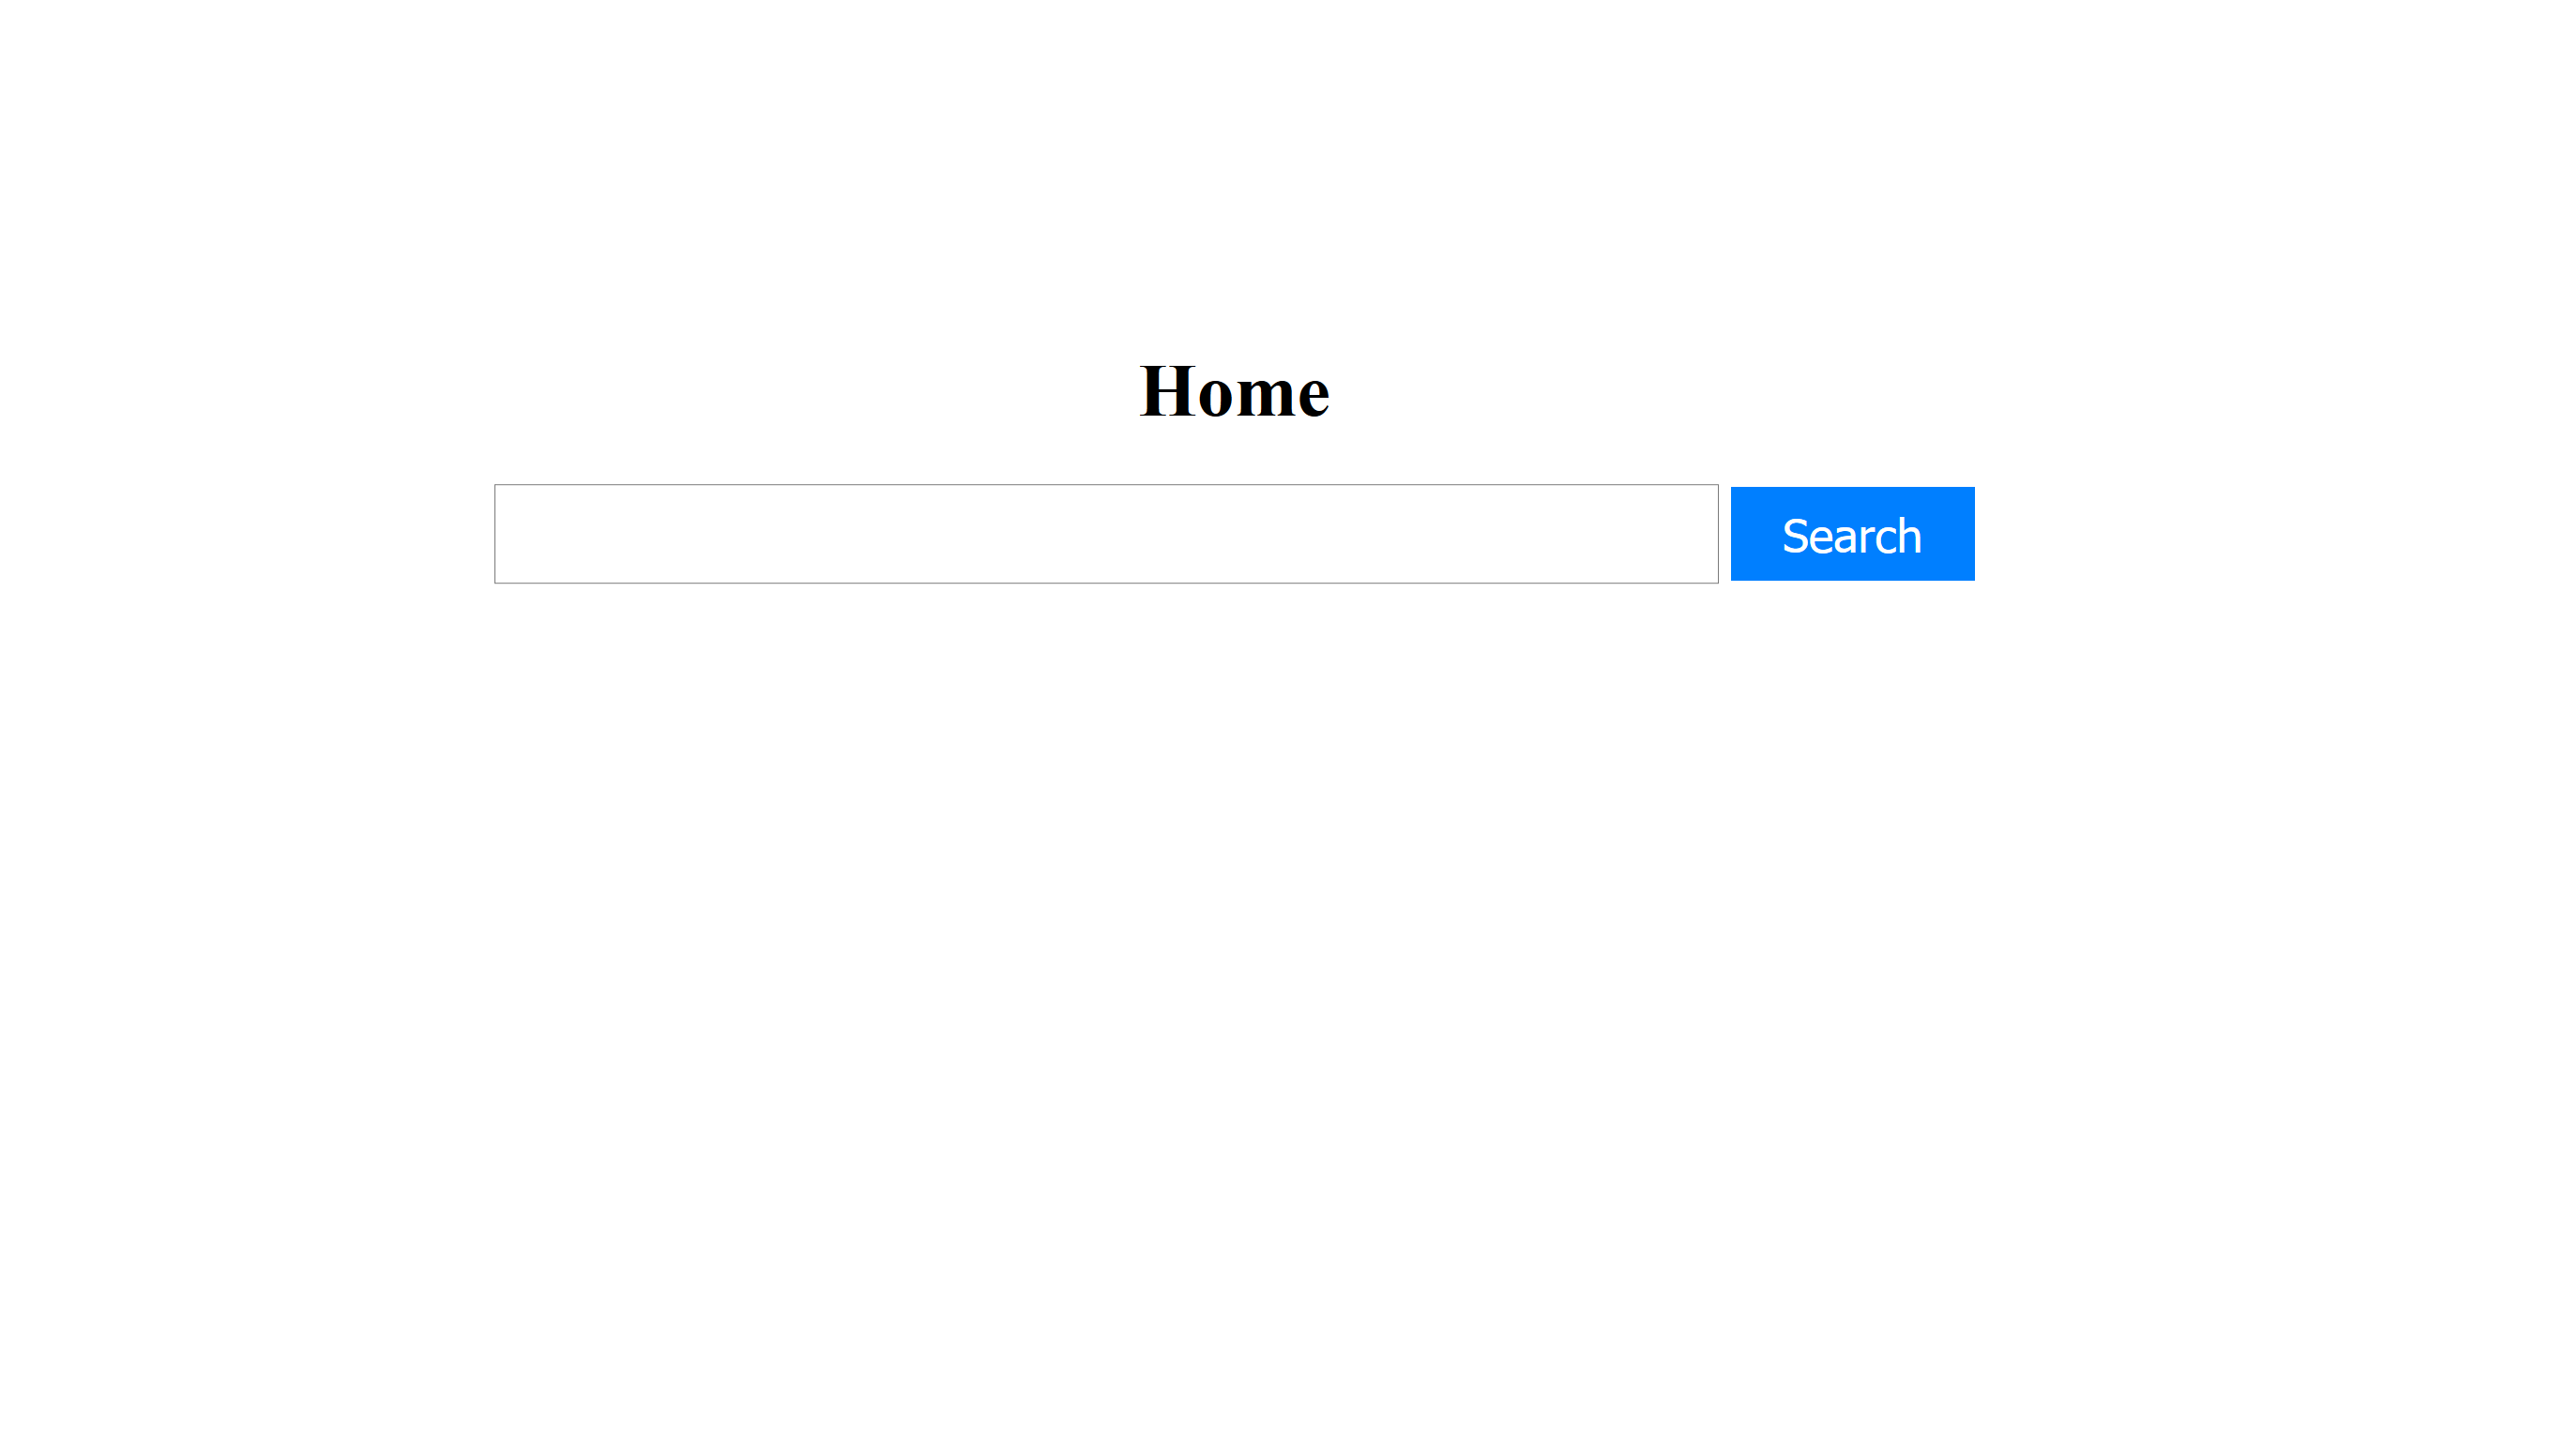
\includegraphics[width=.8\textwidth]{img/1.png}
            \caption{Home}
        \end{figure}
        \begin{figure}[H]
            \centering
            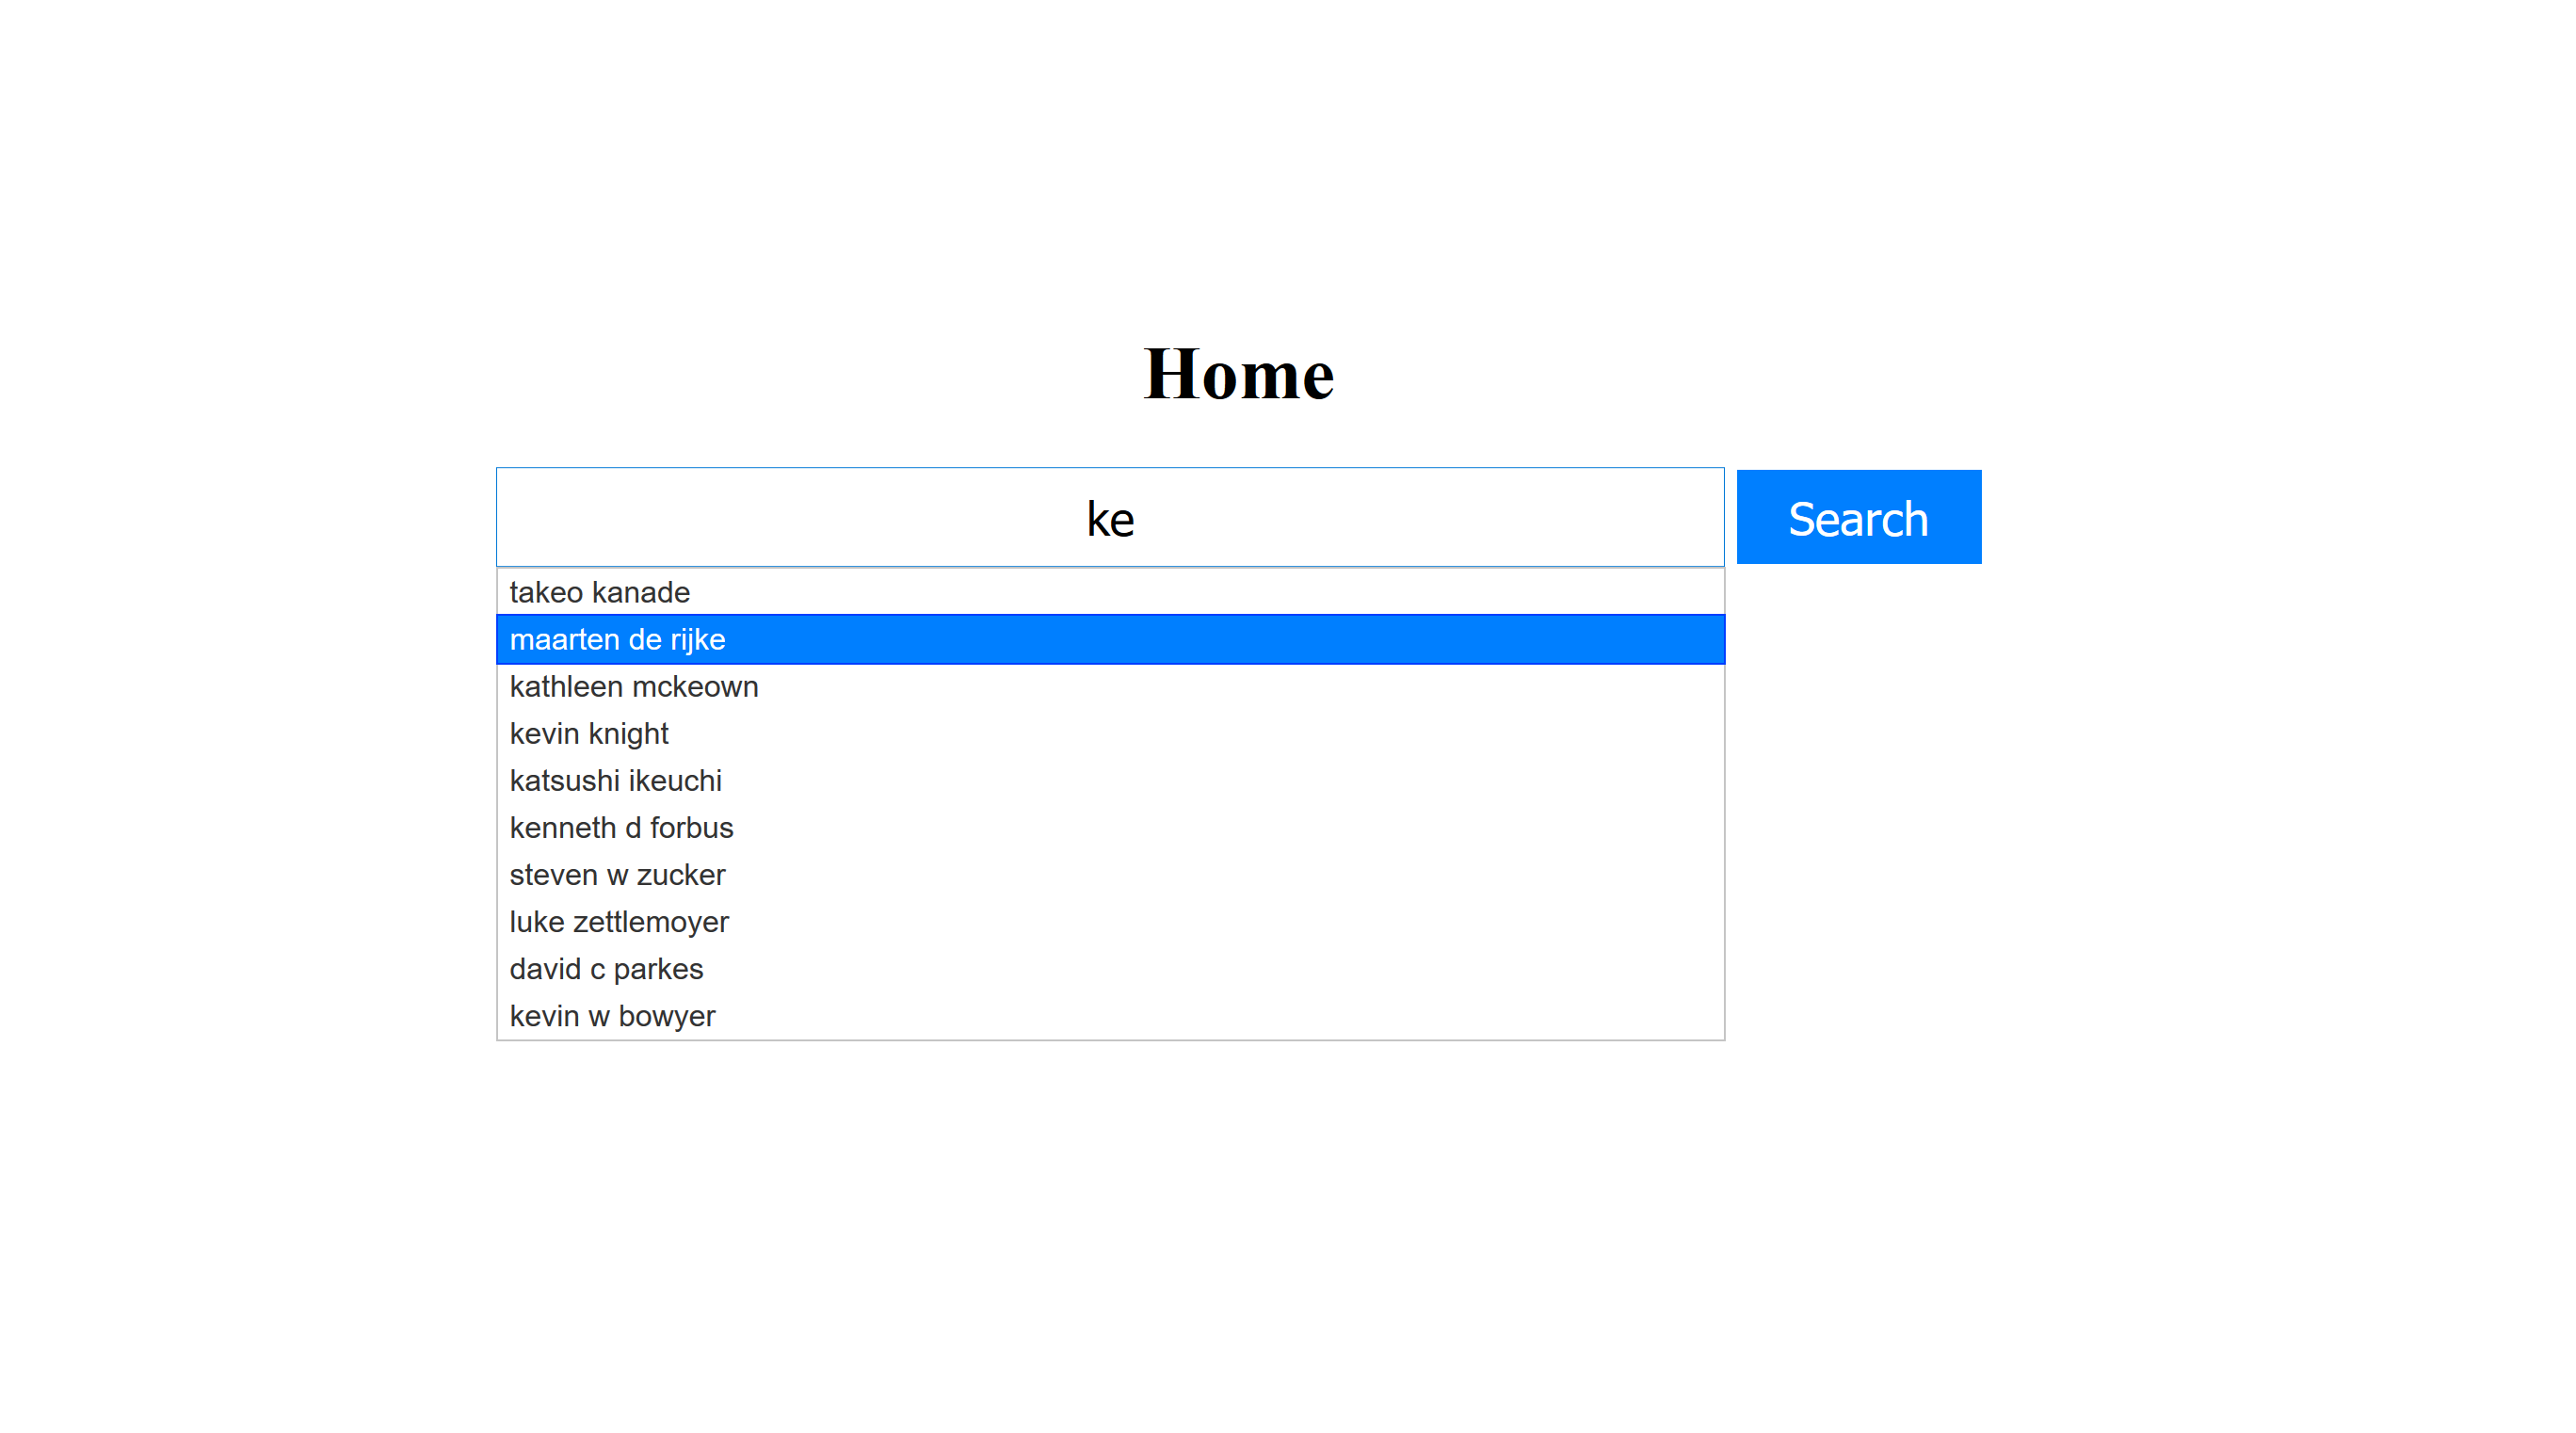
\includegraphics[width=.8\textwidth]{img/2.png}
            \caption{Autocomplete}
        \end{figure}
        \begin{figure}[H]
            \centering
            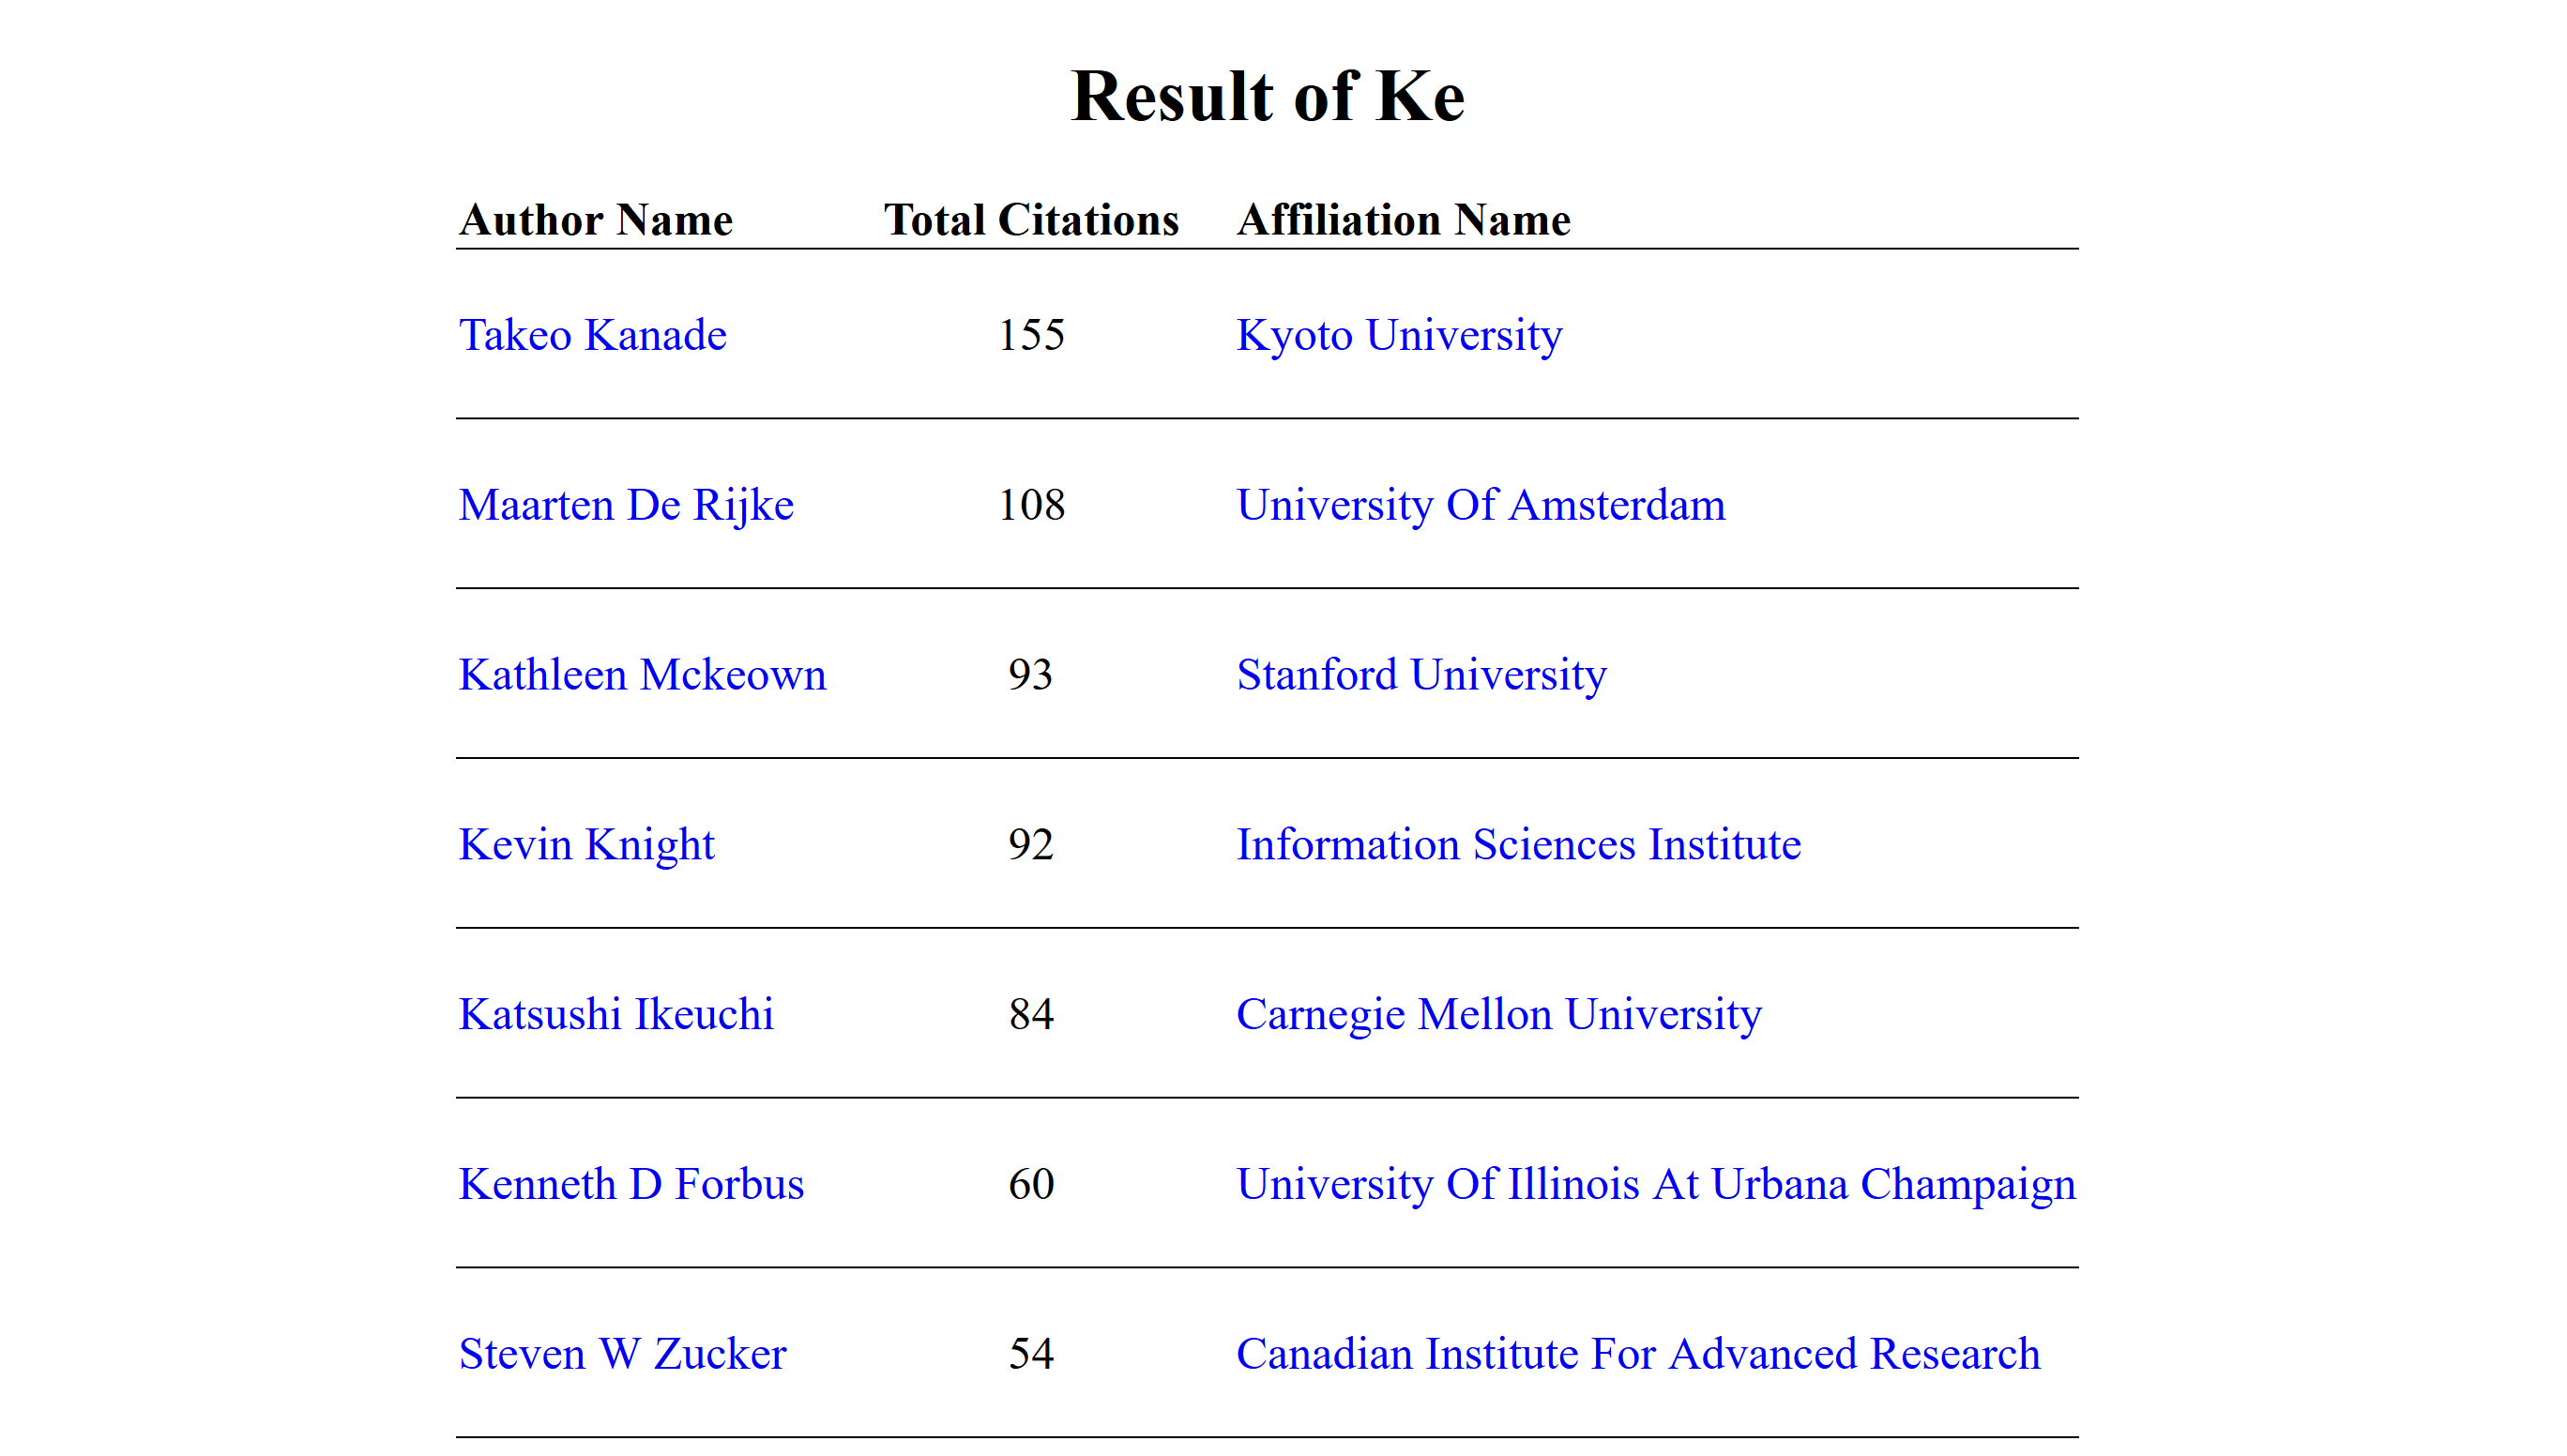
\includegraphics[width=.8\textwidth]{img/3.png}
            \caption{Search Result}
        \end{figure}
        \begin{figure}[H]
            \centering
            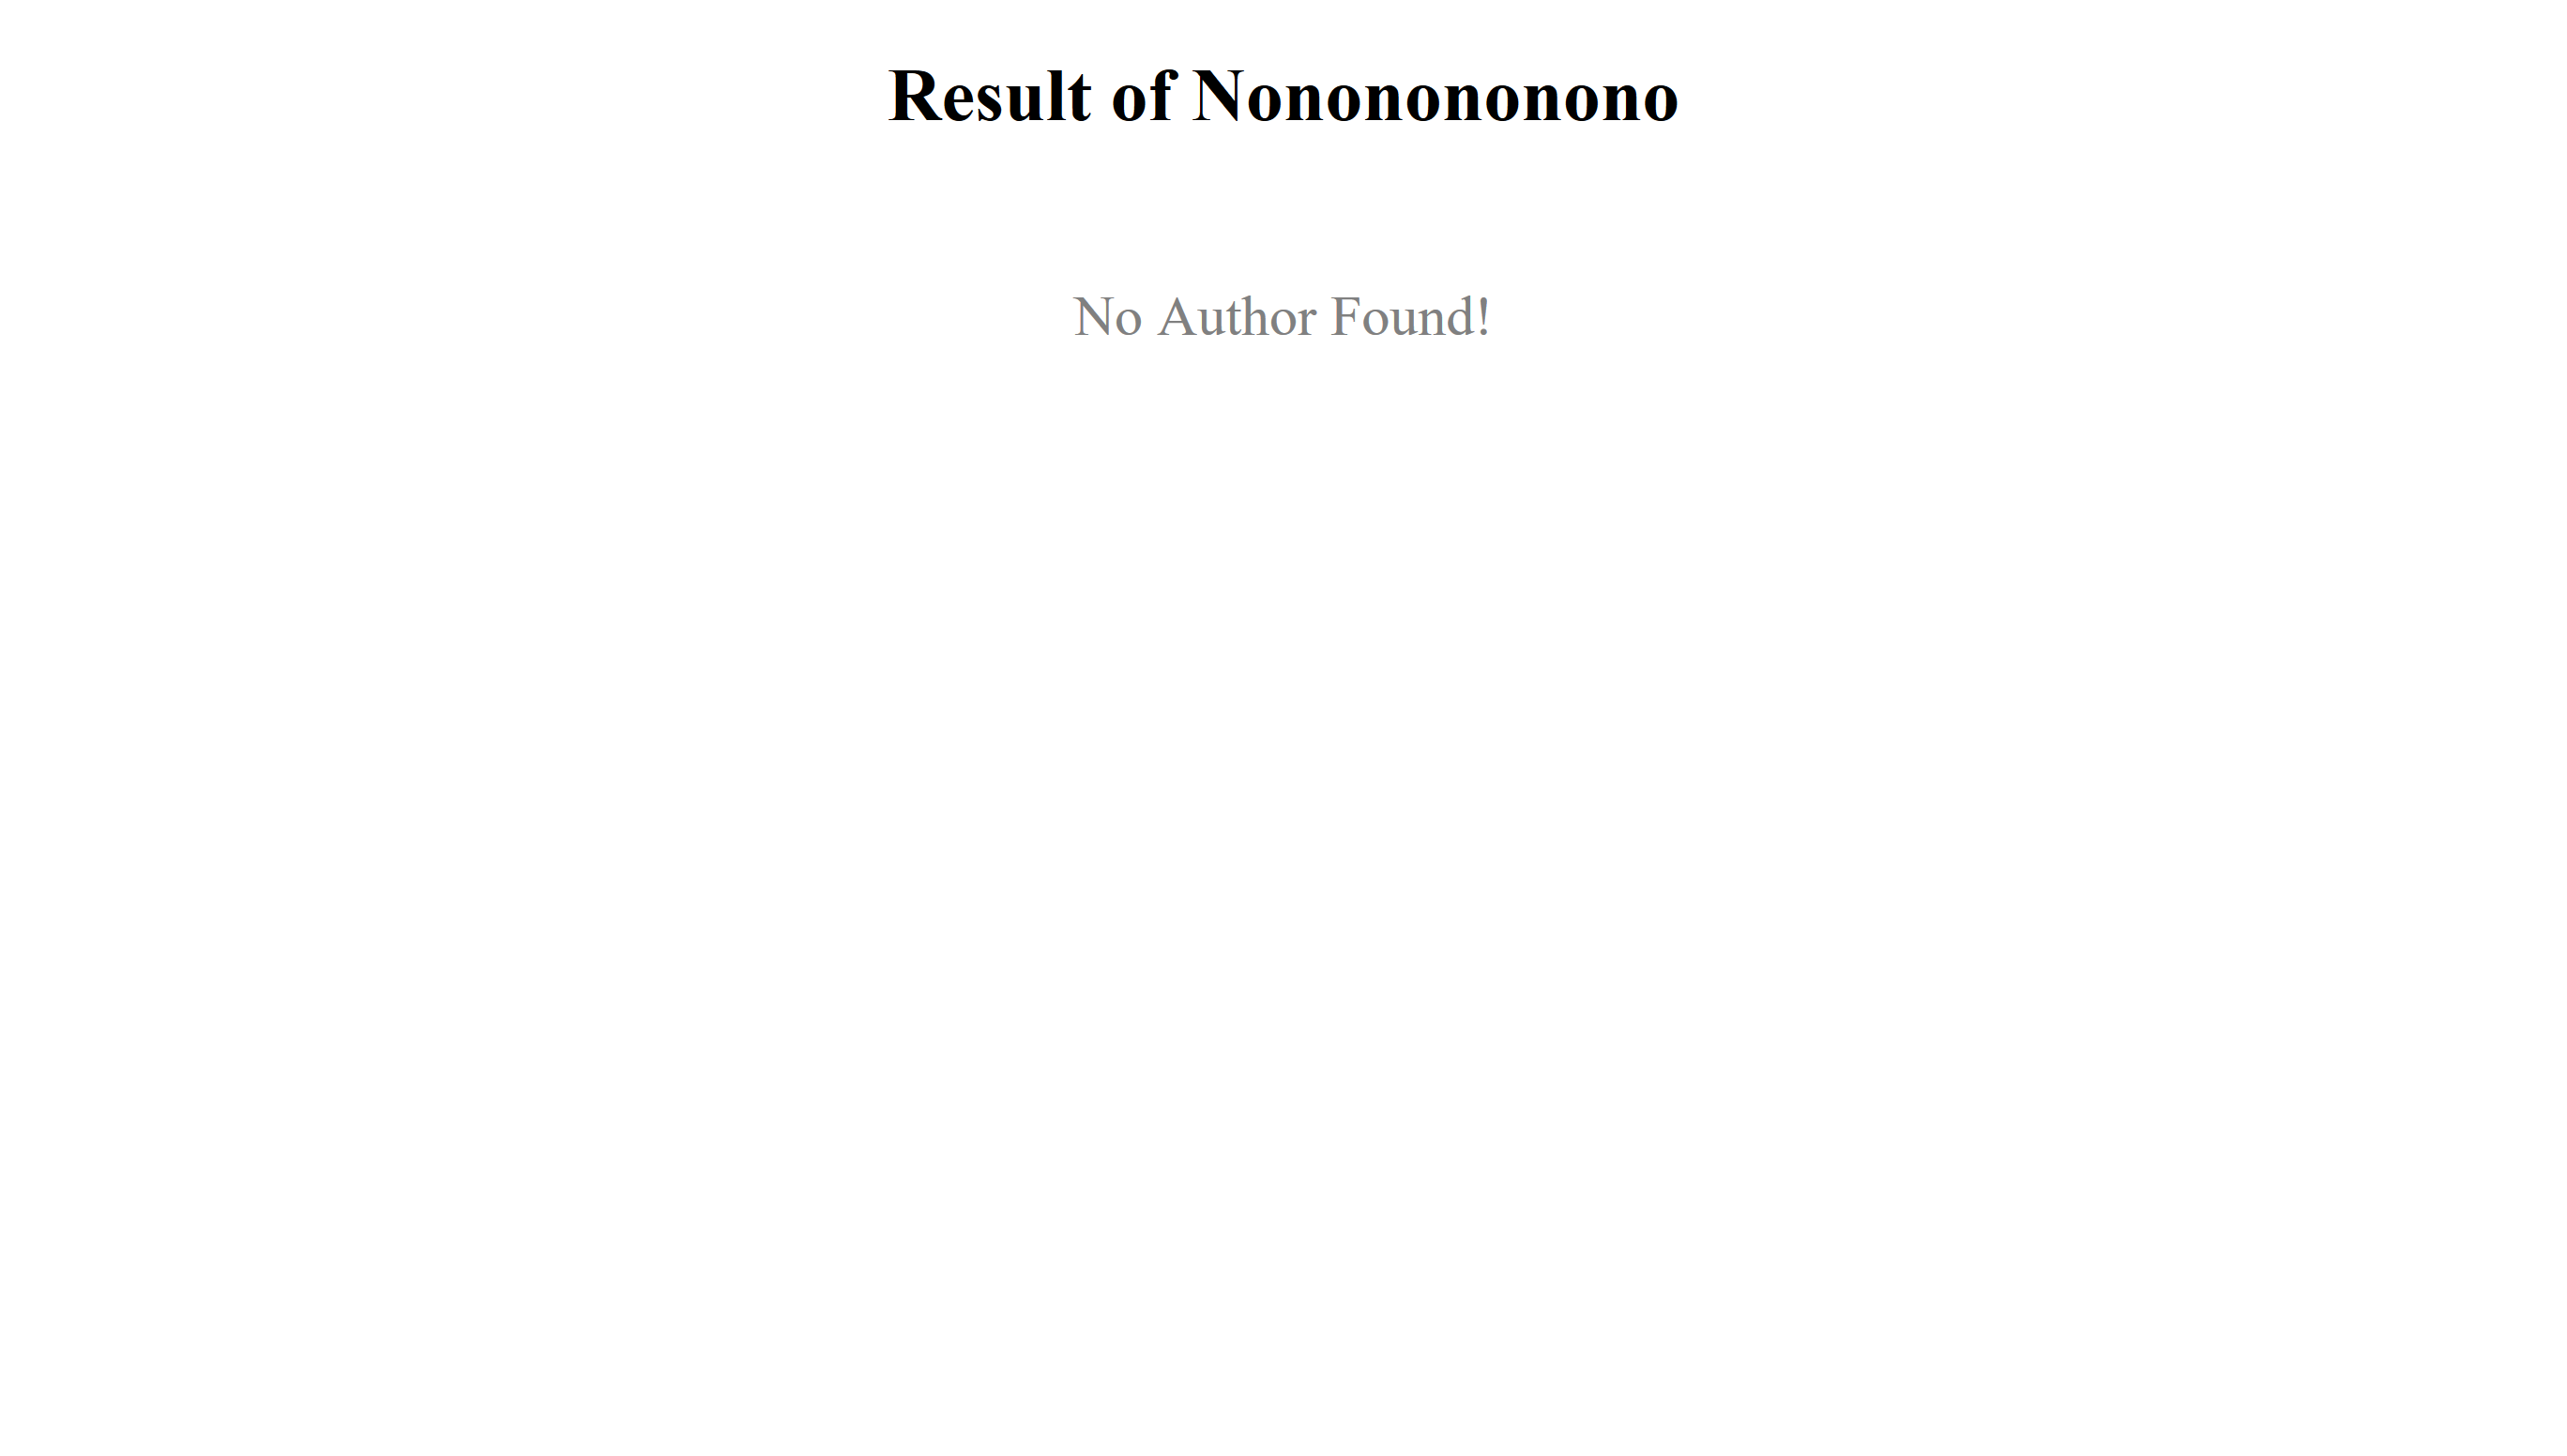
\includegraphics[width=.8\textwidth]{img/4.png}
            \caption{No Result}
        \end{figure}
        \begin{figure}[H]
            \centering
            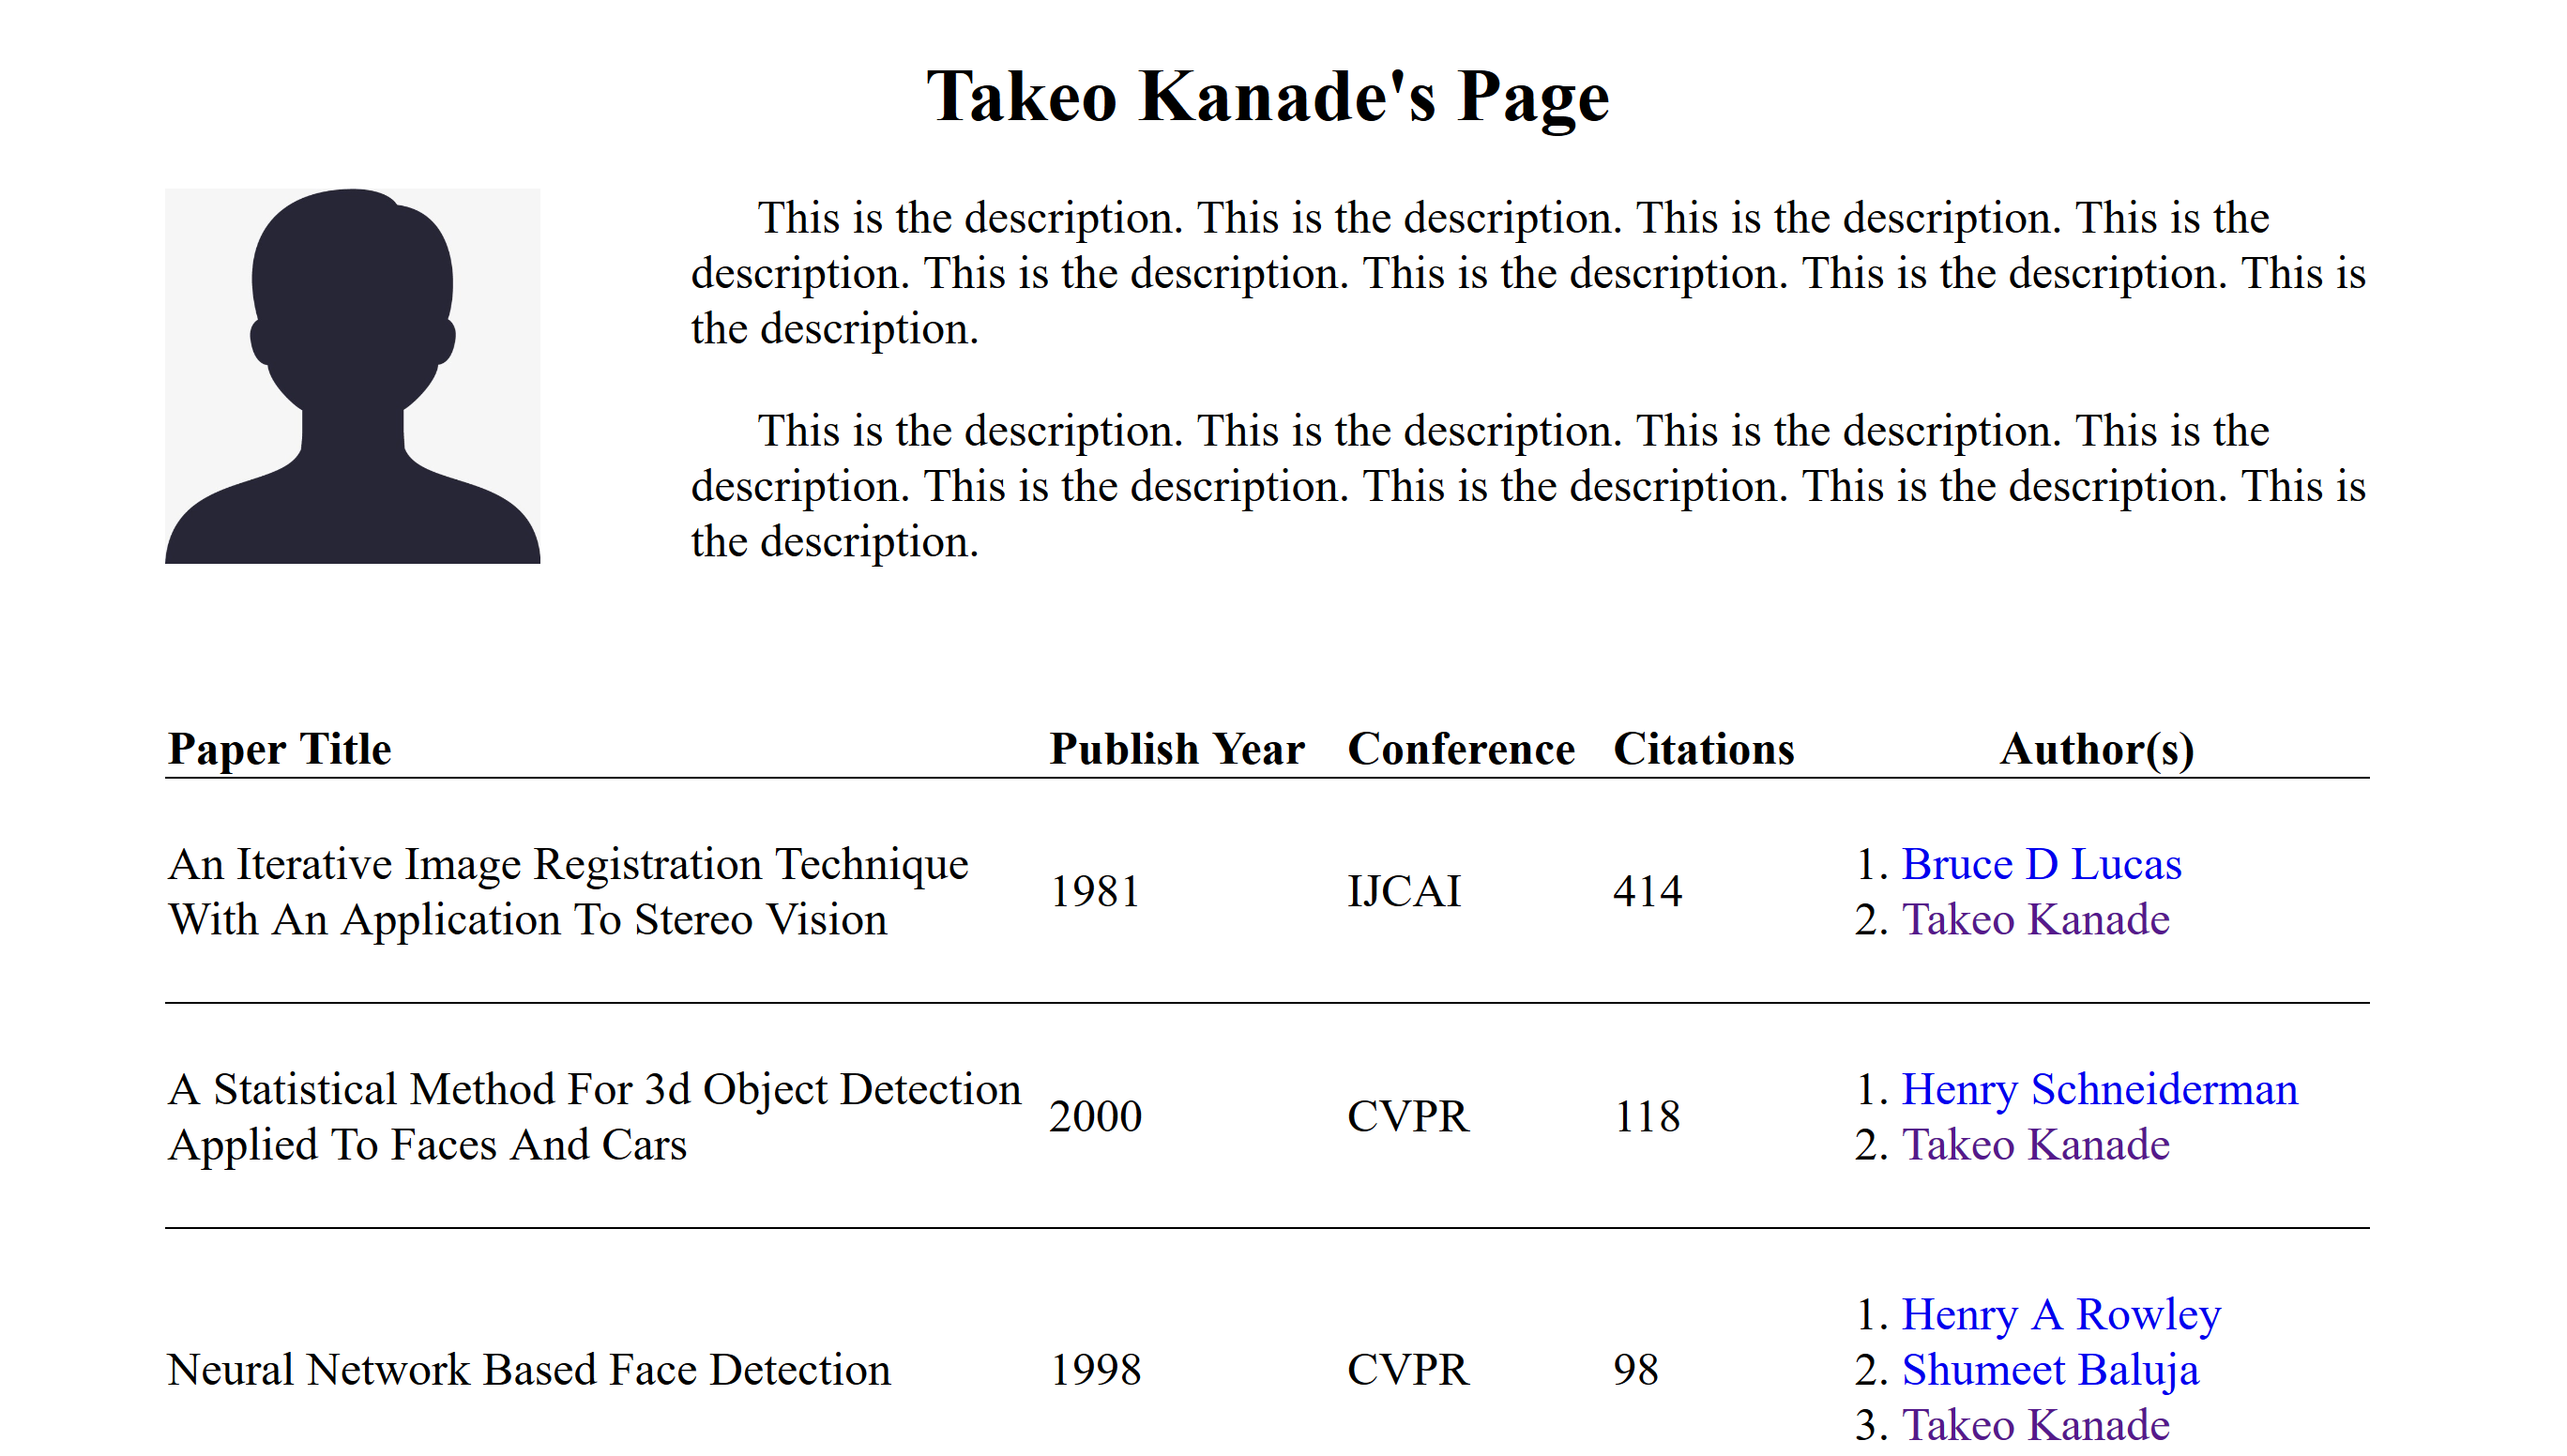
\includegraphics[width=.8\textwidth]{img/5.png}
            \caption{Author}
        \end{figure}
        \begin{figure}[H]
            \centering
            
\includegraphics[width=.8\textwidth]{img/6.png}
            \caption{Invalid Author}
        \end{figure}
    \section{Conclusion And Prospect}
Developing my first PHP website took me quite plenty of time and energy. It's exhausting but worthwhile.

In the process, I got a better understanding of HTML and CSS, which are the basis of frontend. Besides, I learned a new programming language, PHP, which is very useful to develop a website. As for SQL, I also gained a deeper insight into it and learned how to use it effectively.

And when doing the optional Exercise Five, I was introduced to a whole new PHP framework CodeIgniter. The difference and similarity of it and raw PHP are quite impressive.

Eventually, a relatively beautiful and well-built website was developed, much to my delight.

However, to be honest, there're still some improvements for me to make. For example, how to prevent SQL injection? How to prevent XSS and CSRF attack? How to speed up the query more efficiently?

A lot for me to explore!

\end{document}
